\documentclass[prc]{revtex4}
\usepackage[dvips]{graphicx}
\usepackage{mathrsfs}
\usepackage{amsfonts}
\usepackage{lscape}

\usepackage{epic,eepic}
\usepackage{amsmath}
\usepackage{amssymb}
\usepackage[dvips]{epsfig}
\usepackage[T1]{fontenc}
\usepackage{hyperref}
\usepackage{bezier}
\usepackage{pstricks}
\usepackage{dcolumn}% Align table columns on decimal point
\usepackage{bm}% bold math
%\usepackage{braket}
\usepackage[dvips]{graphicx}
\usepackage{pst-plot}

\newcommand{\One}{\hat{\mathbf{1}}}
\newcommand{\eff}{\text{eff}}
\newcommand{\Heff}{\hat{H}_\text{eff}}
\newcommand{\Veff}{\hat{V}_\text{eff}}
\newcommand{\braket}[1]{\langle#1\rangle}
\newcommand{\Span}{\operatorname{sp}}
\newcommand{\tr}{\operatorname{trace}}
\newcommand{\diag}{\operatorname{diag}}
\newcommand{\bra}[1]{\left\langle #1 \right|}
\newcommand{\ket}[1]{\left| #1 \right\rangle}
\newcommand{\element}[3]
    {\bra{#1}#2\ket{#3}}

\newcommand{\normord}[1]{
    \left\{#1\right\}
}

\usepackage{amsmath}
\begin{document}

\title{Exercises FYS4480, week 37, September 12-16, 2022}
%\author{}
\maketitle
\subsection*{Exercise 1}

We will study a schematic model (the Lipkin model, Nucl.
Phys. {\bf 62} (1965) 188) for the interaction among  $4$
fermions that can occupy two different energy levels. Each levels has degeneration $d=4$. The two levels have quantum numbers $\sigma=\pm 1$,
with the upper level having  $\sigma=+1$ and energy
$\varepsilon_{1}=
\varepsilon/2$. The lower level  has $\sigma=-1$ and energy
$\varepsilon_{2}=-\varepsilon/2$. 
In addition, the substates  of each level are characterized  
by the quantum numbers $p=1,2,3,4$.

We define the single-particle states
\[
\ket{u_{\sigma =-1,p}}=a_{-p}^{\dagger}\ket{0}
\hspace{1cm}
\ket{u_{\sigma =1,p}}=a_{+p}^{\dagger}\ket{0}.
\]
The single-particle states span an orthonormal basis.
The Hamiltonian of the system is given by
\[
\begin{array}{ll}
H=&H_{0}+H_{1}+H_{2}\\
&\\
H_{0}=&\frac{1}{2}\varepsilon\sum_{\sigma ,p}\sigma
a_{\sigma,p}^{\dagger}a_{\sigma ,p}\\
&\\
H_{1}=&\frac{1}{2}V\sum_{\sigma ,p,p'}
a_{\sigma,p}^{\dagger}a_{\sigma ,p'}^{\dagger}
a_{-\sigma ,p'}a_{-\sigma ,p}\\
&\\
H_{2}=&\frac{1}{2}W\sum_{\sigma ,p,p'}
a_{\sigma,p}^{\dagger}a_{-\sigma ,p'}^{\dagger}
a_{\sigma ,p'}a_{-\sigma ,p}\\
&\\
\end{array}
\]
where $V$ and $W$ are constants. The operator 
$H_{1}$ can move pairs of fermions as shown in Fig.~(a)
while $H_{2}$ is a spin-exchange term.
As shown in Fig.~(b),
$H_{2}$ moves a pair of fermions from a state $(p\sigma ,p' -\sigma)$ to a state
$(p-\sigma ,p'\sigma)$.
\begin{figure}[hbtp]
\centering
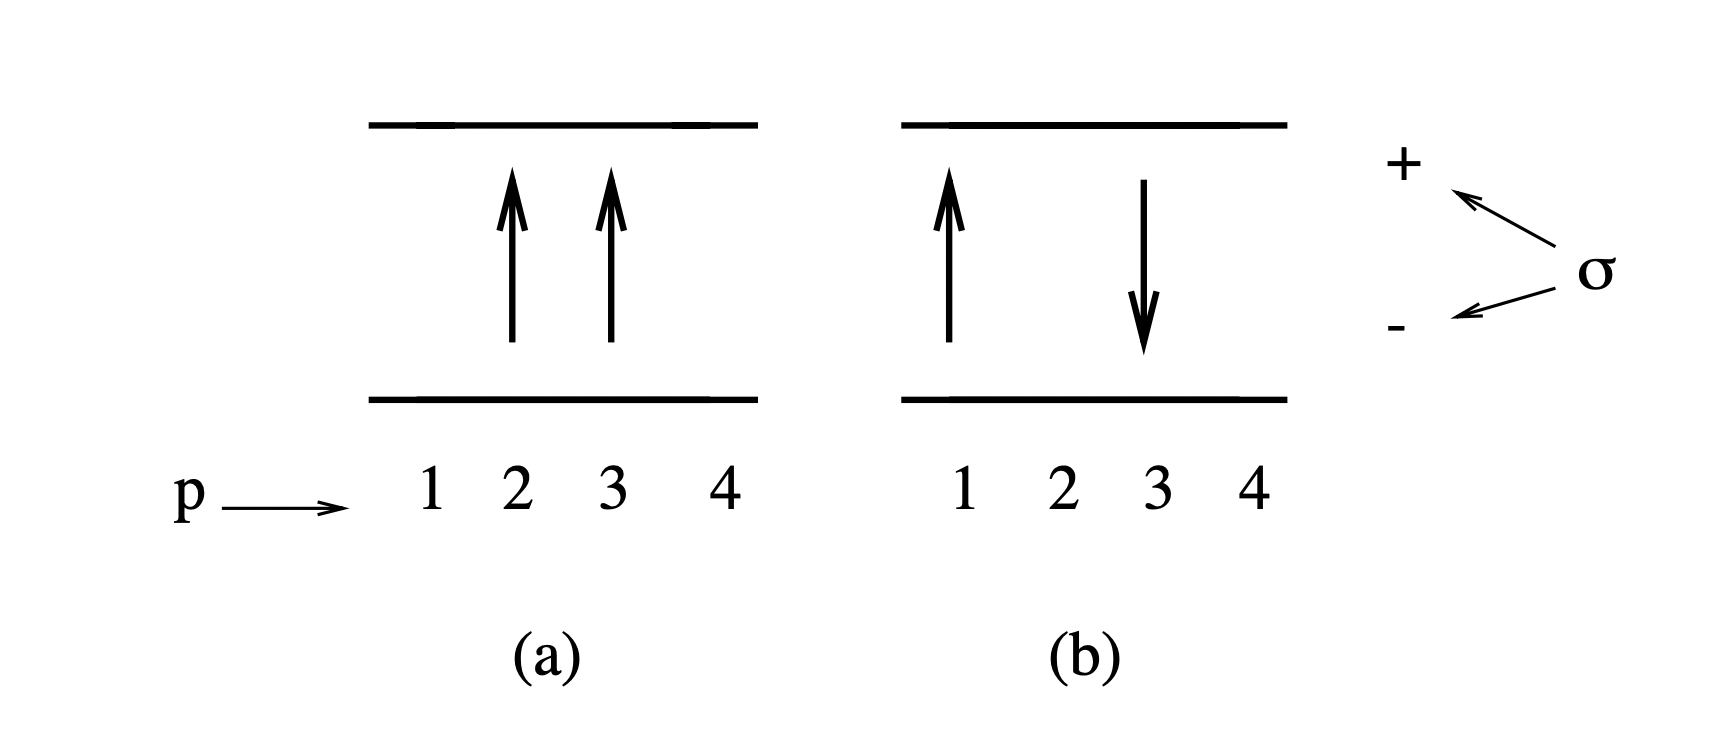
\includegraphics[width=.4\textwidth]{lipkin.png}
\end{figure}

We will encounter this model again in our analysis of the Hartree-fock method. 


\paragraph{Part a)}
Introduce the quasispin operators
\[
\begin{array}{ll}
J_{+}=&\sum_{p}
a_{p+}^{\dagger}a_{p-}\\
&\\
J_{-}=&\sum_{p}
a_{p-}^{\dagger}a_{p+}\\
&\\
J_{z}=&\frac{1}{2}\sum_{p\sigma}\sigma
a_{p\sigma}^{\dagger}a_{p\sigma}\\
&\\
J^{2}=&J_{+}J_{-}+J_{z}^{2}-J_{z}\\
&\\
\end{array}
\]
Show that these operators obey the commutation relations for angular momentum.
\paragraph{Part b)}
Express $H$ in terms of the above quasispin operators and the number operator
\[
N=\sum_{p\sigma}
a_{p\sigma}^{\dagger}a_{p\sigma}.
\]
\paragraph{Part c)}
Show that $H$ commutes with $J^{2}$, viz., $J$ is a good quantum number.
\paragraph{Part d)}
Consider thereafter a state with all four fermions in the lowest level (see the above figure).
We can write this state as
\[
\ket{\Phi_{J_z=-2}} =a_{1-}^{\dagger}a_{2-}^{\dagger}
a_{3-}^{\dagger}a_{4-}^{\dagger}\ket{0}.
\]
This state has $J_{z}=-2$ and belongs to the set of possible projections of 
$J=2$. We introduce the shorthand notation
$\ket{J,J_z}$ for states with different values of
spin $J$ and its projection $J_z$.

The other possible values are  $J_{z}=-1$, $J_{z}=0$, $J_{z}=1$
and $J_{z}=2$. 
Use the ladder operators
$J_{+}$ and $J_{-}$  to set up the states 
with spin $J_{z}=-1$ $J_{z}=0$, $J_{z}=1$
and $J_{z}=2$.  
The action of these operators on a state with given spin 
$J$ and $J_z$ is  (with $\hbar = 1$) 
$J_+\ket{J,J_z}=\sqrt{J(J+1)-J_z(J_z+1)}\ket{J,J_z+1}$ and
$J_-\ket{J,J_z}=\sqrt{J(J+1)-J_z(J_z-1)}\ket{J,J_z-1}$, respectively.

\paragraph{Part e)}
Use thereafter the quasispin operators to construct the Hamiltonian matrix 
$H$ for this five-dimensional space.  Find thereafter the eigenvalues
(numerically using for example Octave or Matlab or python)  for the following parameter sets:
sett av verdier:
\[
\begin{array}{cccc}
(1)&\varepsilon=2,&V=-1/3,&W=-1/4\\
(2)&\varepsilon=2,&V=-4/3,&W=-1
\end{array}
\]
Which state is the ground state? Comment your results.
\end{document}

